\section*{Results}

\begin{table}[htbp]

\begin{tabular}{lllll}
\toprule
{} & samples (RNA) &         Mutations &   Neoantigens & Expressed Neoantigens \\
\midrule
ascites pre-treatment                 &         4 (4) &  10148 $\pm$ 1000 &  199 $\pm$ 60 &           78 $\pm$ 30 \\
ascites post-treatment                &       24 (20) &  13428 $\pm$ 1000 &  295 $\pm$ 50 &          143 $\pm$ 30 \\
\textit{model adjusted change (\%)} &               &       57 $\pm$ 65 &   65 $\pm$ 94 &         117 $\pm$ 142 \\
\hline
solid pre-treatment                   &       76 (70) &    7806 $\pm$ 900 &  152 $\pm$ 20 &            63 $\pm$ 9 \\
solid post-treatment                  &        11 (4) &  11079 $\pm$ 3000 &  264 $\pm$ 90 &           38 $\pm$ 20 \\
\textit{model adjusted change (\%)}   &               &        6 $\pm$ 28 &   11 $\pm$ 41 &          -43 $\pm$ 35 \\
\bottomrule
\end{tabular}

\caption{\textbf{Mean mutations, neoantigens, and expressed noeantigens by sample type and chemotherapy treatment status.} The model-adjusted change is calculated using a Bayesian model that controls for technical variables affecting mutation identification, but does not separate treatment from coincident effects such as surgery and drift. Model effects and means are shown with 95\% credible regions and bootstrapped errors of the mean, respectively.}
\label{tab:cohort}
\end{table}

\begin{figure}[htbp]
\centering
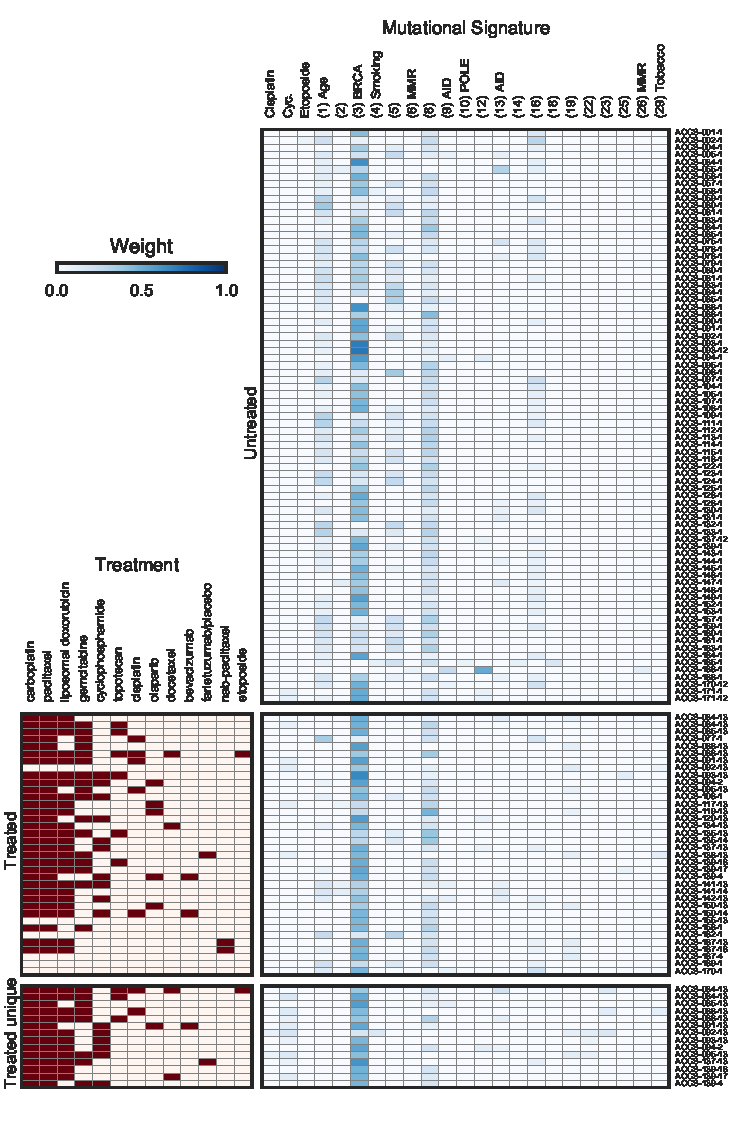
\includegraphics[scale=1.0]{figures/signatures.pdf}
\caption{\textbf{Treatments and mutational signature deconvolutions for paired pre-/post-chemotherapy samples.} \textit{(Top)} Signature deconvolution of the pre-treatment samples. The first five signatures were extracted from reports of a \textit{G. gallus}\cite{Szikriszt_2016} cell line and \textit{C. Elegans}\cite{Meier_2014} organisms after exposure to chemotherapy. The remaining signatures are from the COSMIC signature resource\cite{364242} and give the COSMIC signature number in parentheses. Signatures not shown were undetected in these samples. \textit{(Bottom)} Clinical treatments and signature deconvolutions for the mutations unique to the post-treatment samples. Cases where a chemotherapy signature is detected are annotated by level of agreement with the clinical record. A (*) indicates the donor received the drug (cisplatin and carboplatin are grouped together), and a (?) indicates no record of the donor receiving the drug.}
\label{fig:signatures}
\end{figure}

\begin{figure}[htbp]
\centering
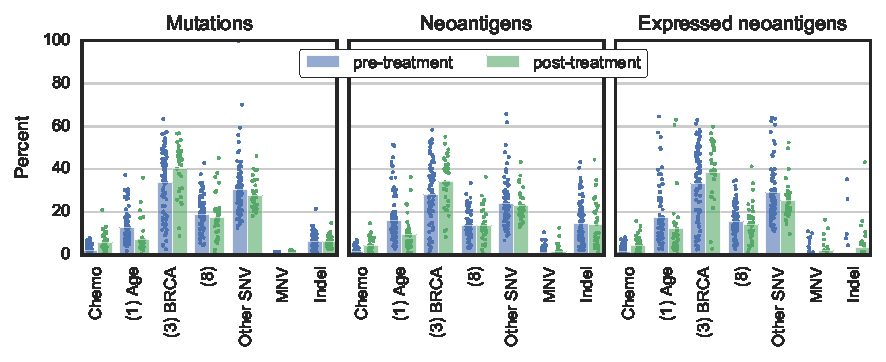
\includegraphics[scale=1.0]{figures/sources_of_mutations_and_neoantigens.pdf}
\caption{\textbf{Sources of mutations and neoantigens:} the estimated fraction of mutations \textit{(left)} and neoantigens \textit{(right)} generated by SNVs from various signatures, multinucleotide variants (MNVs), and indels. The ``chemo'' category combines the SNV signatures extracted from the \textit{G. gallus} and \textit{C. Elegans} studies. COSMIC signature numbers are in parentheses. The ``other'' category shows SNVs from COSMIC signatures other than the ones shown. The ``unclassified'' category shows SNVs that were not accounted for by the signature deconvolution (unknown signatures or a mix of processes). Error bars give the 95\% error of the mean by bootstrapping on samples.}
\label{fig:sources}
\end{figure}

The treated samples showed more mutations, neoantigens, and, in the case of ascites samples, more expressed neoantigens (Table~\ref{tab:cohort}).

Median somatic mutation burden increased post-treatment in 11 of the 12 donors with paired pre- and post-treatment samples (Figure~\ref{fig:supp_paired}). A Bayesian model integrating paired and unpaired samples and controlling for technical variables affecting mutation calling found the post-treatment timepoint to be associated with a 52\% (95\% credible region -1--134) increase in somatic mutations (Figure~\ref{fig:bayesian_model_effects}), with a 93\% posterior probability that post-treatment timepoint was associated with at least a 5\% increase in mutations.

We identified 18,491 potential neoantigens, defined as mutated peptides predicted to bind autologous MHC class I with affinity $\leq 500$nm. All but 26 (0.14\%) neoantigens were private to a single donor. The number of neoantigens tracked the increase in mutational burden after chemotherapy. In the Bayesian analysis, post-treatment samples had 59\% (-15--199) more neoantigens, and, for ascites samples, 106\% (7--305) more expressed neoantigens. Interestingly, solid tumor samples showed an increase in neoantigens but a 44\% (4--67) decrease in expressed neoantigens.

These results describe the observed changes in mutational burden during chemotherapy treatment, but do not isolate the effect of chemotherapy from other effects associated with surgery and relapse. A different model that separately probed the effects of treatment and relapse/recurrence time-point, theoretically possible due to the handful of neoadjuvant-treated donors for whom there are treated primary samples, had large uncertainties and could not rule out that the increase in mutations and neoantigens at relapse may be entirely due non-chemotherapy effects (Figure~\ref{fig:bayesian_model_effects_separate}). We therefore turned to signature deconvolution to assess the extent to which specifically chemotherapy induces mutations.

Signature deconvolution using the 30 mutational signatures curated by COSMIC\cite{364242}, plus four additional signatures extracted from a study of cisplatin-exposed \textit{C. Elegans}\cite{Meier_2014}, and a chicken cell line exposed to cisplatin, cyclophosphamide, and etoposide\cite{Szikriszt_2016} found that the dominant signatures were largely the same in pre- and post-treatment samples (Figure and~\ref{fig:supp_signatures}). In both groups, the top signatures were \textit{Signature 3}, associated with BRCA disruption, \textit{Signature 8}, of unknown etiology, and \textit{Signature 1}, thought to be caused by an endogenous mutational process active across tissues and associated with age at diagnosis. The \textit{G. gallus} cyclophosphamide signature was detected in two pre-treatment samples from the same donor and four post-treatment samples from different donors, three of whom had a clinical record of cyclophosphamide treatment. This signature may have some ability to detect cyclophosphamide treatment but appears to have a substantial false-positive rate. The \textit{G. gallus} etoposide signature was detected in six pre-treatment samples and no post-treatment samples, indicating it has no utility as marker of treatment. The \textit{C. Elegans} cisplatin signature from wildtype worms was not detected in any samples, but the signatures from three genetic knockouts were detected. The \textit{fcd-2} and \textit{xpf-1} knockout signatures each occurred in one cisplatin treated sample and no other samples. The \textit{polq-1} knockout signature seems less useful as marker, appearing in three untreated samples and four carboplatin-treated samples.

For better sensitivity to detect chemotherapy-associated signatures, we next focused on the 14 samples from 12 donors with paired pre- and post-treatment samples. For each donor, we extracted the mutations that had evidence exclusively in the treated samples, requiring at least 30 reads coverage and zero variant reads in the pre-treatment samples. Of 229,132 SNV mutations in the post-treatment samples for these donors, we identified 106,171 such ``unique to treated'' mutations, over which we performed signature deconvolution (Figure ~\ref{fig:signatures}).

The \textit{G. gallus} cisplatin signature, previously undetected in all samples, was found in, and only in, the two cisplatin-treated samples available to this analysis, highlighting its potential utility as a marker of cisplatin (but not carboplatin) exposure. The \textit{C. Elegans} \textit{fcd-2} knockout was detected in three samples, all having received carboplatin but not cisplatin. COSMIC signatures \textit{3} and \textit{8} were detected in 14/14 and 9/14 post-treatment samples, respectively, but \textit{Signature 1} was completely absent, consistent with its association with slow mutagenic processes mostly at work before oncogenesis.

Within the paired samples and considering all chemotherapy-associated signatures except etoposide, at least one chemo signature was detected in 9/14 treated samples and 0/13 untreated samples. The magnitude of the effect of chemo-induced mutagenesis appears typically to be small, however, accounting for less than 12\% of the mutations or neoantigens in 13/14 samples (Figure~\ref{fig:sources}). The exception is sample AOCS-092-13, for which chemo signatures account for 24\% of the mutations and 18\% of the neoantigens. This donor is the most heavily treated in the cohort, having received eight distinct chemotherapeutic agents.
